%%%%%%%%%%%%%%%%%%%%%%%%%%%%%%%%%%%%%%%%%%%%%%%%%%%%%%%%%%%%%%%%%%%%%%%%%%%%%%%
% PREAMBOLO COMUNE PER APPUNTI (Stile Scuro)
%
% Questo file contiene tutte le impostazioni e i pacchetti comuni.
% NON contiene \begin{document} o \end{document}.
%
% Istruzioni per la compilazione del file principale:
% pdflatex -shell-escape nomefile_principale.tex
%%%%%%%%%%%%%%%%%%%%%%%%%%%%%%%%%%%%%%%%%%%%%%%%%%%%%%%%%%%%%%%%%%%%%%%%%%%%%%%

\documentclass{article}

% --- Encoding e lingua ---
\usepackage[utf8]{inputenc}
\usepackage[italian]{babel}

% --- Margini e layout ---
\usepackage{geometry}
\geometry{a4paper, margin=1in}

% --- Font sans-serif (come Helvetica) ---
\usepackage[scaled]{helvet}
\renewcommand{\familydefault}{\sfdefault}
\usepackage[T1]{fontenc}

% --- Matematica ---
\usepackage{amsmath}
\usepackage{amssymb}

% --- Liste personalizzate ---
\usepackage{enumitem}
% \setlist{nosep}

% --- Immagini e Grafica ---
\usepackage{float}
% \usepackage{graphicx}
\usepackage{tikz}
\usetikzlibrary{shapes.geometric, positioning, arrows.meta, calc, fit, backgrounds, patterns, decorations.pathreplacing}

% --- Tabelle Avanzate ---
\usepackage{array}
\usepackage{booktabs}
\usepackage{longtable}

% --- Hyperlink e Metadati PDF ---
\usepackage{hyperref}

\hypersetup{
    colorlinks=true,
    linkcolor=white,
    filecolor=magenta,
    urlcolor=cyan,
    citecolor=green,
    % pdftitle, pdfauthor, ecc. verranno impostati nel file principale
    pdfpagemode=FullScreen,
    bookmarksopen=true,
    bookmarksnumbered=true
}

% --- Licenza del documento ---
\usepackage[
  type={CC},
  modifier={by-sa},
  version={4.0},
]{doclicense}

% --- Colori e Sfondo Nero ---
\usepackage{xcolor}
\pagecolor{black}
\color{white}

% --- Evidenziazione del Codice ---
\usepackage{minted}
\setminted{
    frame=lines,
    framesep=2mm,
    fontsize=\small,
    breaklines=true,
    style=monokai,
    bgcolor=black!80
}
\usemintedstyle{monokai}

% --- Comandi personalizzati per algebra relazionale ---
\newcommand{\Rel}[1]{\textit{#1}} % Per i nomi delle relazioni
\newcommand{\Attr}[1]{\textsf{#1}} % Per i nomi degli attributi

\newcommand{\myunion}{\cup}
\newcommand{\myintersection}{\cap}
\newcommand{\mydifference}{-}
\newcommand{\myrename}[2]{\rho_{#1}(#2)}
\newcommand{\myselectop}[2]{\sigma_{#1}(#2)}
\newcommand{\myproject}[2]{\pi_{#1}(#2)}
\newcommand{\mycartesian}{\times}
\newcommand{\mynaturaljoin}{\bowtie} % Usare \Join da amssymb se disponibile e preferito
\newcommand{\mythetajoin}[3]{#1 \bowtie_{#2} #3} % R1 \bowtie_cond R2

% --- Comandi personalizzati per logica ---
\newcommand{\mylandop}{\wedge}
\newcommand{\myvel}{\vee}
\newcommand{\mynegop}{\neg}
\newcommand{\myforallop}{\forall}
\newcommand{\myexistsop}{\exists}

% --- Join esterni (outer join) ---
% Definizione standard per i join esterni
\def\ojoin{\setbox0=\hbox{$\mynaturaljoin$}%
	\rule[-.02ex]{.25em}{.4pt}\llap{\rule[\ht0]{.25em}{.4pt}}}
\newcommand{\myleftouterjoin}{\mathbin{\ojoin\mkern-5.8mu\mynaturaljoin}}
\newcommand{\myrightouterjoin}{\mathbin{\mynaturaljoin\mkern-5.8mu\ojoin}}
\newcommand{\myfullouterjoin}{\mathbin{\ojoin\mkern-5.8mu\mynaturaljoin\mkern-5.8mu\ojoin}}



% --- Titolo ---
\title{Appunti di Reti di Calcolatori}
\author{Basato sulle slide del Prof. Luciano Bononi}
\date{\today}

\begin{document}

\maketitle
\tableofcontents
\newpage

\section{Reti di Reti e Internetworking}
\begin{itemize}
    \item \textbf{Concetto Base:} Le reti locali (LAN) individuali sono interconnesse per formare reti più grandi. Questa interconnessione avviene in modo gerarchico.
    \item \textbf{Componenti Chiave:}
    \begin{itemize}
        \item \textbf{Router:} Calcolatori specializzati che collegano diverse LAN (o sottoreti). Ogni router è un ``rappresentante'' della sua rete locale.
        \item \textbf{Backbone (Dorsali):} Linee dati ad alta velocità che collegano i router tra loro.
    \end{itemize}
    \item \textbf{Astrazione a Livello Rete (Livello 3 OSI):}
    \begin{itemize}
        \item Dal punto di vista di un router, i dettagli interni delle LAN collegate sono nascosti. Il router vede solo altri router e le reti che questi rappresentano.
        \item Questo è fondamentale per la \textbf{scalabilità}: invece di dover conoscere l'indirizzo MAC (livello 2) di ogni singolo dispositivo su Internet, un router deve solo sapere come raggiungere la \textit{rete} di destinazione, inoltrando il pacchetto al router successivo appropriato.
        \item \textbf{Esempio Pratico:} Immagina il sistema postale. Il postino del tuo quartiere (router locale) non ha bisogno di conoscere l'indirizzo esatto di ogni casa in un'altra città. Sa solo che deve mandare la lettera al centro di smistamento di quella città (router di backbone o router della rete di destinazione), che poi si occuperà della consegna locale.
    \end{itemize}
    \begin{figure}[H]
        \centering
        \includegraphics[width=0.8\textwidth]{images/reti_di_reti.png}
        \caption{Diagramma Reti di Reti}
    \end{figure}
    \item \textbf{Problema Risolto:} Se milioni di computer fossero connessi solo con switch e bridge (livello 2), l'instradamento dei frame richiederebbe tabelle MAC enormi, causando ritardi, complessità e rischi di errore. I router, operando al livello 3 (Rete), semplificano questo gestendo l'instradamento tra reti.
\end{itemize}

\section{Livello Rete: Internet Protocol (IP)}
Il concetto di rete si estende dalla LAN locale alla rete globale (Internet).
\begin{itemize}
    \item \textbf{Protocollo Internet (IP):}
    \begin{itemize}
        \item \textbf{Indirizzamento IP:} Introduce un nuovo schema di indirizzamento globale e gerarchico.
        \begin{itemize}
            \item Fornisce indirizzi alla rete locale e ai suoi nodi (host).
        \end{itemize}
        \item \textbf{Instradamento (Forwarding):} Gestisce l'inoltro dei pacchetti dal mittente al destinatario finale.
        \begin{itemize}
            \item Servizio di comunicazione di tipo \textbf{connectionless} (senza connessione preliminare, ogni pacchetto è trattato indipendentemente).
        \end{itemize}
        \item \textbf{Nuovi Dispositivi (Router):} Amministratori del livello 3.
        \begin{itemize}
            \item \textbf{Tabelle di instradamento:} Illustrano la topologia della rete (dal punto di vista del router), nascondendo i dettagli interni delle LAN.
            \item \textbf{Protocolli di routing:} Protocolli per aggiornare dinamicamente le tabelle di instradamento (vedi sezione successiva).
        \end{itemize}
        \item \textbf{Frammentazione:} Suddivide i dati in pacchetti più piccoli se necessario per attraversare reti con Maximum Transmission Unit (MTU) diverse.
        \item \textbf{Busta del Pacchetto (Header IP):} Contiene gli indirizzi IP del mittente e del destinatario e altre informazioni di controllo.
    \end{itemize}
    \item \textbf{Collocazione nello Stack ISO/OSI (o Internet Stack):}
    \begin{itemize}
        \item Livello Fisico (es. codifica segnali)
        \item Livello Data Link (MAC/LLC, es. Ethernet, Wi-Fi, PPP) - accesso al mezzo, controllo errore locale.
        \item \textbf{Livello Rete (IP)} - frammentazione, indirizzamento, instradamento.
        \item Livello Trasporto (TCP/UDP)
        \item Livelli superiori (Sessione, Presentazione, Applicazione)
    \end{itemize}
\end{itemize}

\section{Indirizzamento IPv4}
\begin{itemize}
    \item \textbf{Indirizzi IP:} Identificatori unici per le interfacce di rete (schede di rete) connesse a Internet.
    \begin{itemize}
        \item Un dispositivo con più schede di rete può avere più indirizzi IP.
        \item \textbf{Associazione MAC-IP:} Un indirizzo IP è associato a un indirizzo MAC.
        \begin{itemize}
            \item \textbf{IP Statico:} L'associazione non cambia (configurato manualmente).
            \item \textbf{IP Dinamico:} L'associazione può cambiare (assegnato da un server, es. DHCP).
        \end{itemize}
    \end{itemize}
    \item \textbf{Formato IPv4:}
    \begin{itemize}
        \item 32 bit (4 Byte).
        \item Rappresentato come 4 valori decimali separati da punti (es. \texttt{192.168.1.10}).
        \item Ogni valore decimale è compreso tra 0 e 255.
        \item \textbf{Esempio:} \texttt{130.136.25.1}
    \end{itemize}
    \item \textbf{Struttura dell'Indirizzo IP:}
    \begin{itemize}
        \item \textbf{Network Number (Numero di Rete):} Identifica la rete IP a cui appartiene l'interfaccia.
        \item \textbf{Host Number (Numero dell'Host):} Identifica l'interfaccia specifica all'interno di quella rete.
    \end{itemize}
    \item \textbf{Classi di Reti IPv4 (obsolete ma didatticamente utili):}
    \begin{itemize}
        \item Il valore del primo byte determina la classe.
        \item \textbf{Classe A:}
        \begin{itemize}
            \item Primo bit: \texttt{0} (valori primo byte: 1-126).
            \item Formato: \texttt{0NNNNNNN.HHHHHHHH.HHHHHHHH.HHHHHHHH}
            \item Poche reti (max 126), ma ognuna con moltissimi host (oltre 16 milioni).
            \item Esempio: \texttt{10.0.0.1} (Rete \texttt{10.0.0.0})
        \end{itemize}
        \item \textbf{Classe B:}
        \begin{itemize}
            \item Primi due bit: \texttt{10} (valori primo byte: 128-191).
            \item Formato: \texttt{10NNNNNN.NNNNNNNN.HHHHHHHH.HHHHHHHH}
            \item Numero medio di reti (max 16.382), ognuna con molti host (oltre 64.000).
            \item Esempio: \texttt{172.16.0.1} (Rete \texttt{172.16.0.0})
        \end{itemize}
        \item \textbf{Classe C:}
        \begin{itemize}
            \item Primi tre bit: \texttt{110} (valori primo byte: 192-223).
            \item Formato: \texttt{110NNNNN.NNNNNNNN.NNNNNNNN.HHHHHHHH}
            \item Moltissime reti (oltre 2 milioni), ma ognuna con pochi host (max 254).
            \item Esempio: \texttt{192.168.1.1} (Rete \texttt{192.168.1.0})
        \end{itemize}
    \end{itemize}
    \textit{(Nota: L'indirizzamento classful è stato ampiamente sostituito da Classless Inter-Domain Routing (CIDR), ma la comprensione delle classi aiuta a capire la logica originale.)}
\end{itemize}

\section{Sottoreti (Subnetwork)}
\begin{itemize}
    \item \textbf{Scopo:} Organizzare ulteriormente una rete IP in segmenti più piccoli e gestibili.
    \item \textbf{Subnet Mask (Maschera di Sottorete):}
    \begin{itemize}
        \item Valore a 32 bit che definisce la parte (sotto)rete e la parte host.
        \item Bit a \texttt{1} = parte (sotto)rete; Bit a \texttt{0} = parte host.
        
        \begin{figure}[H]
            \centering
            \begin{tikzpicture}[scale=0.9]
                % First draw colored rectangles
                \fill[blue!20] (0,1) rectangle (3,2);
                \fill[green!20] (3,1) rectangle (4,2);
                \fill[blue!20] (0,0) rectangle (3,1);
                \fill[green!20] (3,0) rectangle (4,1);
                
                % Then draw grid on top
                \draw[thick] (0,1) grid (4,2);
                \draw[thick] (0,0) grid (4,1);
                
                % Add labels on top of everything
                \node at (-1.5,1.5) {\textcolor{primarytext}{Indirizzo IP:}};
                \node at (0.5,1.5) {\textcolor{black}{192}};
                \node at (1.5,1.5) {\textcolor{black}{168}};
                \node at (2.5,1.5) {\textcolor{black}{1}};
                \node at (3.5,1.5) {\textcolor{black}{10}};
                
                \node at (-1.5,0.5) {\textcolor{primarytext}{Subnet Mask:}};
                \node at (0.5,0.5) {\textcolor{black}{255}};
                \node at (1.5,0.5) {\textcolor{black}{255}};
                \node at (2.5,0.5) {\textcolor{black}{255}};
                \node at (3.5,0.5) {\textcolor{black}{0}};
                
                % Legenda
                \draw[fill=blue!20] (5,1.5) rectangle (5.5,2);
                \node[anchor=west] at (5.7,1.75) {\textcolor{primarytext}{Parte Rete}};
                \draw[fill=green!20] (5,0.5) rectangle (5.5,1);
                \node[anchor=west] at (5.7,0.75) {\textcolor{primarytext}{Parte Host}};
            \end{tikzpicture}
            \caption{Separazione Rete/Host con Subnet Mask}
        \end{figure}

        \begin{table}[H]
            \centering
            \begin{tabular}{|c|c|c|c|}
                \hline
                \textbf{Notazione CIDR} & \textbf{Subnet Mask} & \textbf{Bit Rete} & \textbf{Host Disponibili} \\
                \hline
                /24 & 255.255.255.0 & 24 & 254 \\
                /25 & 255.255.255.128 & 25 & 126 \\
                /26 & 255.255.255.192 & 26 & 62 \\
                /27 & 255.255.255.224 & 27 & 30 \\
                /28 & 255.255.255.240 & 28 & 14 \\
                \hline
            \end{tabular}
            \caption{Esempi di Subnet Mask Comuni}
        \end{table}

        \item \textbf{Calcolo dell'Indirizzo di Rete:} Si applica l'operazione logica AND bit a bit tra l'indirizzo IP e la subnet mask:
        
        \begin{figure}[H]
            \centering
            \begin{tabular}{rcl}
                IP: & 192.168.1.10 & = \textcolor{themeblue}{11000000.10101000.00000001}.\textcolor{green}{00001010} \\
                Mask: & 255.255.255.0 & = \textcolor{themeblue}{11111111.11111111.11111111}.\textcolor{green}{00000000} \\
                \hline
                AND & & \\
                \hline
                Rete: & 192.168.1.0 & = \textcolor{themeblue}{11000000.10101000.00000001}.\textcolor{green}{00000000} \\
            \end{tabular}
            \caption{Esempio di Calcolo dell'Indirizzo di Rete}
        \end{figure}
        
        \item \textbf{Divisione tra Rete e Host:} In un indirizzo IP con subnet mask:
        
        \begin{itemize}
            \item La parte \textcolor{themeblue}{colorata in blu} rappresenta la \textbf{porzione di rete} (network portion)
            \item La parte \textcolor{green}{colorata in verde} rappresenta la \textbf{porzione di host}
        \end{itemize}
        
        Nell'esempio sopra con subnet mask /24 (255.255.255.0):
        \begin{itemize}
            \item I primi 24 bit (\textcolor{themeblue}{3 ottetti}) identificano la rete
            \item Gli ultimi 8 bit (\textcolor{green}{1 ottetto}) identificano l'host all'interno della rete
        \end{itemize}
        
        \item \textbf{Altro Esempio (con classi di reti):}
        \begin{itemize}
            \item Rete Classe B: \texttt{130.136.0.0} (Netmask di classe: \texttt{255.255.0.0})
            \item Con netmask \texttt{255.255.255.0} per 256 sottoreti:
            \begin{itemize}
                \item \texttt{130.136.1.0} è la sottorete 1.
                \item \texttt{130.136.1.22} è l'host 22 sulla sottorete \texttt{130.136.1.0}.
            \end{itemize}
        \end{itemize}
    \end{itemize}
    
    \begin{figure}[H]
        \centering
        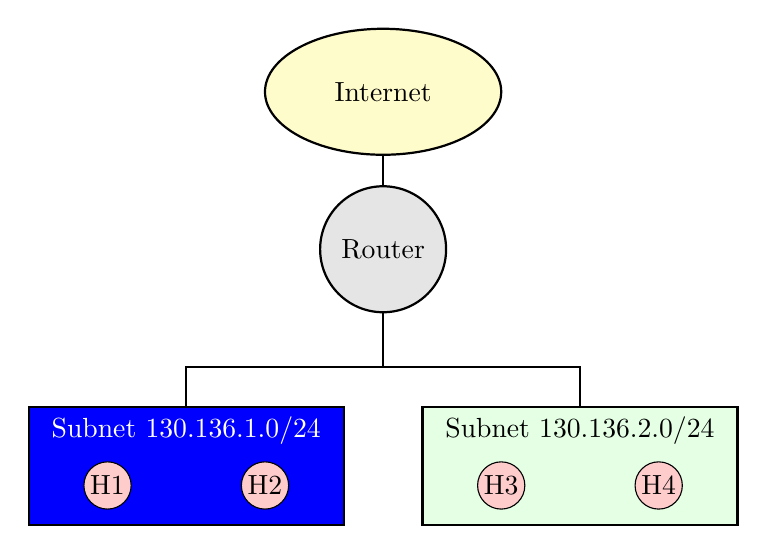
\begin{tikzpicture}[scale=1.0]
            % Router principale
            \draw[thick,fill=gray!20] (0,0) circle (0.8) node {\textcolor{black}{Router}};
            
            % Subnet 1
            \draw[thick,fill=blue] (-4.5,-2) rectangle (-0.5,-3.5);
            \node at (-2.5,-2.3) {\textcolor{white}{Subnet 130.136.1.0/24}};
            \draw[fill=red!20] (-3.5,-3) circle (0.3) node {\textcolor{black}{H1}};
            \draw[fill=red!20] (-1.5,-3) circle (0.3) node {\textcolor{black}{H2}};
            
            % Subnet 2
            \draw[thick,fill=green!10] (0.5,-2) rectangle (4.5,-3.5);
            \node at (2.5,-2.3) {\textcolor{black}{Subnet 130.136.2.0/24}};
            \draw[fill=red!20] (1.5,-3) circle (0.3) node {\textcolor{black}{H3}};
            \draw[fill=red!20] (3.5,-3) circle (0.3) node {\textcolor{black}{H4}};
            
            % Connessioni
            \draw[thick] (0,-0.8) -- (0,-1.5);
            \draw[thick] (0,-1.5) -- (-2.5,-1.5) -- (-2.5,-2);
            \draw[thick] (0,-1.5) -- (2.5,-1.5) -- (2.5,-2);
            
            % Router Internet
            \draw[thick,fill=yellow!20] (0,2) ellipse (1.5 and 0.8) node {\textcolor{black}{Internet}};
            \draw[thick] (0,0.8) -- (0,1.2);
        \end{tikzpicture}
        \caption{Esempio di Rete Suddivisa in Sottoreti}
    \end{figure}
    
    \item \textbf{Gerarchia di Sottoreti:} Ogni sottorete è amministrata da un router (\textbf{default router} o default gateway).
    \item \textbf{Informazioni di Configurazione Fondamentali per un Host:}
    \begin{enumerate}
        \item Indirizzo IP
        \item Subnet Mask (\textit{Netmask} o \textit{Maschera di Sottorete})
        \item Default Gateway (\textit{Router di default})
    \end{enumerate}
\end{itemize}

\section{Instradamento (Forwarding) dei Pacchetti IP}
\begin{itemize}
    \item \textbf{Forwarding:} Processo decisionale di un router per inoltrare un pacchetto IP.
    \item \textbf{Routing Table:} Ogni router ha una tabella con reti di destinazione e "next hop".
    \item \textbf{Processo (Esempio Semplificato):}
    \begin{enumerate}
        \item Un host (\texttt{H1}) invia un pacchetto a un host (\texttt{H2}) su un'altra rete.
        \item \texttt{H1} invia il pacchetto al suo default router (\texttt{R1}).
        \item \texttt{R1} controlla l'IP di destinazione e consulta la sua tabella:
        \begin{itemize}
            \item Se rete direttamente connessa, inoltra a \texttt{H2} (via ARP).
            \item Altrimenti, inoltra al router "next hop" (\texttt{R2}).
        \end{itemize}
        \item \texttt{R2} ripete il processo, e così via fino alla destinazione.
    \end{enumerate}
    \item \textbf{Esempio Completo:} Host \texttt{140.217.2.10} (rete Y) spedisce a \texttt{130.136.2.33} (rete K).
    
    \begin{figure}[H]
        \centering
        \includegraphics[width=1\textwidth]{images/percorso_pacchetto.png}
        \caption{Percorso di un pacchetto IP attraverso diverse reti}
    \end{figure}
    
    \begin{enumerate}
        \item Pacchetto a default router di \texttt{Y.2} (\texttt{Ry2: 140.217.2.254}).
        \item \texttt{Ry2} inoltra a default router di rete \texttt{Y} (\texttt{Ry: 140.217.0.254}).
        \item \texttt{Ry} inoltra a \texttt{Rz} (\texttt{190.89.0.254}).
        \item \texttt{Rz} inoltra a \texttt{Rk} (\texttt{130.136.0.254}).
        \item \texttt{Rk} inoltra a router sottorete \texttt{K.2} (\texttt{Rk2: 130.136.2.254}).
        \item \texttt{Rk2} consegna a host \texttt{130.136.2.33}.
    \end{enumerate}
\end{itemize}

\section{Routing}
\begin{itemize}
    \item \textbf{Routing vs. Forwarding:}
    \begin{itemize}
        \item \textbf{Forwarding:} Azione di spostare pacchetti basata su tabella esistente.
        \item \textbf{Routing:} Processo di costruzione e aggiornamento delle tabelle di instradamento.
    \end{itemize}
    \item \textbf{Esempio di Tabella di Routing (Router Rz):}
    \begin{table}[H]
        \centering
        \begin{tabular}{|l|l|l|c|}
            \hline
            \textbf{Rete Destinazione} & \textbf{Netmask} & \textbf{Next Hop} & \textbf{Interfaccia} \\
            \hline
            190.89.0.0 & 255.255.0.0 & 0.0.0.0 & eth0 \\
            \hline
            130.136.0.0 & 255.255.0.0 & 130.136.0.254 & eth1 \\
            \hline
            140.217.0.0 & 255.255.0.0 & 140.217.0.254 & eth2 \\
            \hline
            192.168.5.0 & 255.255.255.0 & 192.168.5.254 & eth3 \\
            \hline
            0.0.0.0 & 0.0.0.0 & 203.15.16.1 & eth4 \\
            \hline
        \end{tabular}
        \caption{Esempio di Tabella di Routing del Router Rz}
    \end{table}
    \begin{itemize}
        \item Interpretazione della tabella:
        \begin{itemize}
            \item Per la rete 190.89.0.0 (rete locale): consegna diretta (next hop 0.0.0.0)
            \item Per la rete 130.136.0.0 (rete K): inoltra a 130.136.0.254 (Rk)
            \item Per la rete 140.217.0.0 (rete Y): inoltra a 140.217.0.254 (Ry)
            \item Per la rete 192.168.5.0: inoltra al router 192.168.5.254
            \item Per tutte le altre destinazioni (0.0.0.0/0): inoltra al gateway predefinito 203.15.16.1
        \end{itemize}
    \end{itemize}
    \item \textbf{Necessità di Aggiornamento Tabelle:} Cambiamenti topologia, mobilità, accordi tra Sistemi Autonomi (AS).
    \begin{itemize}
        \item \textbf{AS (Autonomous System):} Rete/insieme di reti sotto una singola amministrazione tecnica.
    \end{itemize}
    \item \textbf{Protocolli di Routing (Algoritmi):}
    \begin{itemize}
        \item I router li usano per scambiarsi informazioni e calcolare percorsi migliori.
        \item \textbf{Esempi:}
        \begin{itemize}
            \item \textbf{RIP (Routing Information Protocol)}
            \item \textbf{OSPF (Open Shortest Path First)} (IGP - Interior Gateway Protocol)
            \item \textbf{BGP (Border Gateway Protocol)} (EGP - Exterior Gateway Protocol)
        \end{itemize}
    \end{itemize}
\end{itemize}

\section{Protocollo ICMP (Internet Control Message Protocol)}
\begin{itemize}
    \item \textbf{Scopo:} Protocollo per messaggi di controllo e di errore; non trasporta dati utente.
    \item \textbf{Funzionamento:} Opera a fianco di IP; messaggi ICMP incapsulati in pacchetti IP.
    \item \textbf{Tipi di Messaggi Comuni:}
    \begin{itemize}
        \item Rete/Host destinazione non raggiungibile/sconosciuto
        \item Protocollo richiesto non disponibile
        \item Echo Request / Echo Reply (usato da \texttt{PING})
        \item Time Exceeded (TTL arrivato a zero, usato da \texttt{Traceroute})
    \end{itemize}
\end{itemize}

\section{Applicazioni Basate su ICMP}
\begin{itemize}
    \item \textbf{PING (Packet InterNet Groper):}
    \begin{itemize}
        \item \textbf{Scopo:} Testare la connettività.
        \item \textbf{Funzionamento:} \texttt{host1} invia ICMP Echo Request a \texttt{host2}; \texttt{host2} risponde con ICMP Echo Reply. Calcola RTT.
        \item \textbf{Esempio di Comando:}
\begin{minted}{bash}
bitrey@amella-laptop:~$ ping virtuale.unibo.it -c 4
\end{minted}
        \item \textbf{Output Esempio:}
\begin{minted}{text}
PING frontend-http-azure-01.unibo.it (51.124.58.146) 56(84) bytes of data.
64 bytes from 51.124.58.146: icmp_seq=1 ttl=116 time=50.9 ms
64 bytes from 51.124.58.146: icmp_seq=2 ttl=116 time=50.6 ms
64 bytes from 51.124.58.146: icmp_seq=3 ttl=116 time=50.7 ms
64 bytes from 51.124.58.146: icmp_seq=4 ttl=116 time=50.2 ms

--- frontend-http-azure-01.unibo.it ping statistics ---
4 packets transmitted, 4 received, 0% packet loss, time 3006ms
rtt min/avg/max/mdev = 50.153/50.606/50.928/0.286 ms
bitrey@amella-laptop:~$ 
\end{minted}
        \item \textbf{Interpretazione dell'Output:}
        \begin{itemize}
            \item \texttt{bytes}: Dimensione del pacchetto ICMP
            \item \texttt{icmp\_seq}: Numero di sequenza del pacchetto
            \item \texttt{ttl}: Time To Live del pacchetto (decrementato ad ogni router)
            \item \texttt{time}: Round Trip Time (RTT) in millisecondi
            \item \texttt{statistics}: Sommario con percentuale di pacchetti persi e statistiche RTT
        \end{itemize}
        \item \textbf{Utilità:} Diagnostica problemi di rete, misura latenza, verifica raggiungibilità
    \end{itemize}
    \item \textbf{Traceroute (o \texttt{tracert} su Windows):}
    \begin{itemize}
        \item \textbf{Scopo:} Mostrare la sequenza di router attraversati.
        \item \textbf{Funzionamento:} Invia pacchetti con TTL crescente. Ogni router che fa scadere il TTL invia ICMP Time Exceeded.
        \item \textbf{Output Esempio:}
\begin{minted}{text}
Rilevazione instradamento verso mi-bo-g.garr.net [193.206.134.21]
1 <1 ms <1 ms <1 ms csgw-3-0-5.cs.unibo.it [130.136.2.254]
2 <1 ms <1 ms <1 ms cesia-csgw.cs.unibo.it [130.136.254.254]
...
5  4 ms  4 ms  4 ms mi-bo-g.garr.net [193.206.134.21]
\end{minted}
    \end{itemize}
\end{itemize}


\section{Protocollo ARP (Address Resolution Protocol) e RARP}
\label{sec:arp_combined}

Il protocollo \textbf{ARP} (\textit{Address Resolution Protocol}) è un protocollo di rete fondamentale che opera al livello 2 (Data Link) del modello OSI. Il suo \textbf{problema} principale da risolvere è il seguente: per inviare un frame Ethernet (o un altro tipo di frame di livello datalink) all'interno di una rete locale (LAN), un host necessita dell'indirizzo MAC (Media Access Control) del destinatario, ma spesso conosce solo il suo indirizzo IP.

\subsection{Funzionamento del Protocollo ARP}
ARP permette di trovare l'indirizzo MAC corrispondente a un dato indirizzo IP sulla stessa LAN. Il meccanismo si basa su un meccanismo di richiesta-risposta che coinvolge due tipi di messaggi:
\begin{enumerate}
    \item Il mittente (Host A), non conoscendo il MAC del destinatario (es. Host B con IP\_B), invia un \textbf{ARP Request} in \textit{broadcast} (indirizzo MAC di destinazione FF:FF:FF:FF:FF:FF) a tutti i dispositivi sulla LAN. La richiesta è del tipo: ``Chi ha l'indirizzo IP\_B? Per favore, inviami il tuo indirizzo MAC.''
    \item L'host che possiede l'IP\_B (Host B) riceve la richiesta e risponde con un \textbf{ARP Reply} in \textit{unicast} direttamente all'Host A. La risposta contiene l'associazione IP\_B $\leftrightarrow$ MAC\_B richiesta.
\end{enumerate}
Una volta ricevuta la risposta, il mittente (Host A) memorizza l'associazione IP-MAC nella sua \textbf{ARP Cache} (o ARP table) per un certo periodo di tempo. Questo evita di ripetere la richiesta per comunicazioni future con lo stesso host. Anche l'Host B può aggiornare la sua ARP Cache con le informazioni dell'Host A. Le voci nella cache possono essere dinamiche (con un tempo di scadenza) o statiche (configurate manualmente e permanenti).

\begin{figure}[H]
    \centering
    % Assicurati che il percorso dell'immagine sia corretto
    \includegraphics[width=0.6\textwidth]{images/arp_simulation.png}
    \caption{Funzionamento del protocollo ARP: Host A invia un ARP Request per l'IP di Host B. Host B risponde con un ARP Reply contenente il suo MAC.}
    \label{fig:arp_simulation_combined}
\end{figure}

\subsection{Esempio di Tabella ARP}
\begin{table}[H]
    \centering
    \label{tab:arp_cache_example_combined}
    \begin{tabular}{|l|l|l|c|}
        \hline
        \rowcolor{bg_custom}
        \textbf{Indirizzo IP} & \textbf{Indirizzo MAC} & \textbf{Tipo} & \textbf{Tempo Residuo} \\
        \hline
        192.168.1.1 & 00:11:22:33:44:55 & Statico & Permanente \\
        \hline
        192.168.1.5 & AA:BB:CC:DD:EE:FF & Dinamico & 110 sec \\
        \hline
        192.168.1.10 & 11:22:33:44:55:66 & Dinamico & 587 sec \\
        \hline
    \end{tabular}
    \caption{Esempio di Tabella ARP su un host}
\end{table}

\subsection{Vantaggi e Limitazioni di ARP}
\begin{description}
    \item[Vantaggi:]
    \begin{itemize}[nosep]
        \item \textbf{Automatizzazione:} Risoluzione automatica degli indirizzi MAC senza configurazione manuale.
        \item \textbf{Efficienza:} Il caching delle associazioni riduce il traffico di richieste ripetute.
        \item \textbf{Semplicità:} Protocollo leggero e di facile implementazione.
    \end{itemize}
    \item[Limitazioni:]
    \begin{itemize}[nosep]
        \item \textbf{Sicurezza:} Vulnerabile ad attacchi (es. ARP spoofing, cache poisoning) data l'assenza di autenticazione.
        \item \textbf{Scalabilità:} Limitato alle reti locali (non attraversa i router).
        \item \textbf{Overhead:} Le richieste broadcast possono generare traffico significativo in reti estese.
    \end{itemize}
\end{description}

\subsection{Considerazioni sulla Sicurezza}
Le vulnerabilità intrinseche di ARP lo espongono a rischi:
\begin{itemize}[nosep]
    \item \textbf{ARP Spoofing/Cache Poisoning:} Un attaccante invia ARP Reply falsificati per associare il proprio MAC all'IP di un'altra vittima (es. il gateway), intercettando o reindirizzando il traffico.
    \item \textbf{Denial of Service (DoS):} Invio massiccio di ARP Request o Reply per saturare la rete o le tabelle ARP degli host.
\end{itemize}
Contromisure includono: voci ARP statiche, \textit{Dynamic ARP Inspection} (DAI) sugli switch gestiti, e protocolli di sicurezza come \textit{Secure ARP} (S-ARP), sebbene quest'ultimo sia poco diffuso.

\subsection{RARP (Reverse Address Resolution Protocol)}
\textbf{RARP} aveva lo scopo opposto di ARP: permetteva a un host di scoprire il proprio indirizzo IP conoscendo il proprio indirizzo MAC. Era utilizzato principalmente da dispositivi diskless (senza disco fisso) durante la fase di avvio. RARP è stato in gran parte sostituito da protocolli più robusti e flessibili come BOOTP e, soprattutto, \textbf{DHCP} (Dynamic Host Configuration Protocol).

\vspace{0.5cm}
\noindent Nonostante le sue limitazioni, in particolare quelle di sicurezza, il protocollo ARP rimane un componente essenziale per il funzionamento delle reti IP su LAN, garantendo la comunicazione trasparente tra dispositivi nella stessa rete locale.


\section{Assegnazione Indirizzi IP: DHCP (Dynamic Host Configuration Protocol)}
\begin{itemize}
    \item \textbf{Scopo:} Automatizzare l'assegnazione di IP e altre info di configurazione.
    \item \textbf{Server DHCP:} Gestisce un pool di IP e li assegna dinamicamente ai client.
    \begin{itemize}
        \item \textbf{Informazioni fornite:} IP, netmask, gateway, DNS.
    \end{itemize}
    \item \textbf{Processo DHCP (semplificato - DORA):}
    \begin{enumerate}
        \item \textbf{Discover:} Client (broadcast): ``Cerco server DHCP.''
        \item \textbf{Offer:} Server(s) DHCP: ``Posso darti IP X.''
        \item \textbf{Request:} Client: ``Accetto IP X dal server Y.''
        \item \textbf{Acknowledge:} Server Y: ``OK, IP X è tuo per N ore.''
    \end{enumerate}
    
    \begin{figure}[H]
        \centering
        \includegraphics[width=0.9\textwidth]{images/dhcp_process.png}
        \caption{Processo DHCP (DORA): Discover, Offer, Request, Acknowledge}
    \end{figure}
    
\begin{table}[H]
    \centering
    \begin{tabular}{|l|p{9cm}|}
        \hline
        \rowcolor{bg_custom}
        \textbf{Informazione Configurata} & \textbf{Esempio e Descrizione} \\
        \hline
        Indirizzo IP & \textcolor{primarytext}{\texttt{192.168.1.10} - Identificatore univoco per l'host} \\
        \hline
        Subnet Mask & \textcolor{primarytext}{\texttt{255.255.255.0} - Definisce la porzione rete dell'IP} \\
        \hline
        Default Gateway & \textcolor{primarytext}{\texttt{192.168.1.1} - Router per raggiungere altre reti} \\
        \hline
        DNS Server & \textcolor{primarytext}{\texttt{8.8.8.8, 8.8.4.4} - Server per risolvere nomi in IP} \\
        \hline
        Lease Time & \textcolor{primarytext}{\texttt{86400 secondi} (24 ore) - Durata dell'assegnazione} \\
        \hline
        WINS Server & \textcolor{primarytext}{\texttt{192.168.1.100} - Per risoluzione nomi NetBIOS (Windows)} \\
        \hline
        NTP Server & \textcolor{primarytext}{\texttt{pool.ntp.org} - Server per sincronizzazione oraria} \\
        \hline
    \end{tabular}
    \caption{Informazioni tipiche fornite da un server DHCP}
  \end{table}
  
  \begin{table}[H]
    \centering
    \begin{tabular}{|l|p{9cm}|}
        \hline
        \rowcolor{bg_custom}
        \textbf{Caratteristiche} & \textbf{Descrizione} \\
        \hline
        Scope & \textcolor{primarytext}{Intervallo di indirizzi che il server può assegnare (es. 192.168.1.10-192.168.1.100)} \\
        \hline
        Esclusioni & \textcolor{primarytext}{Indirizzi nell'ambito che non devono essere assegnati (es. 192.168.1.20-192.168.1.25)} \\
        \hline
        Static IPs & \textcolor{primarytext}{Associazioni fisse MAC-IP per dispositivi specifici (es. server, stampanti)} \\
        \hline
        Lease Time & \textcolor{primarytext}{Durata dell'assegnazione, dopo la quale il client deve rinnovare} \\
        \hline
        Opzioni DHCP & \textcolor{primarytext}{Informazioni addizionali come DNS, gateway, ecc.} \\
        \hline
    \end{tabular}
    \caption{Concetti base nella configurazione di un server DHCP}
  \end{table}
  
    \item \textbf{Vantaggi:} Semplifica amministrazione, evita conflitti, uso efficiente IP.
\end{itemize}

\section{IPv6 e Tunnelling IPv4}
\begin{itemize}
    \item \textbf{Motivazioni per IPv6:} Esaurimento indirizzi IPv4.
    \item \textbf{Caratteristiche Salienti di IPv6:}
    \begin{itemize}
        \item \textbf{Indirizzi IPv6 Estesi:} \textbf{128 bit} (16 Byte). Numero enorme di indirizzi.
        \item \textbf{Nuova Struttura dell'Header IP.}
    \end{itemize}
    \item \textbf{Integrazione/Sostituzione di IPv4:}
    \begin{itemize}
        \item Transizione graduale. Tecniche come Dual Stack.
        \item \textbf{Tunnelling:} Spedire pacchetti IPv6 incapsulati in pacchetti IPv4 attraverso una rete IPv4.
    \end{itemize}
\end{itemize}

\section{Livello Trasporto (TCP e UDP)}
\begin{itemize}
    \item \textbf{Scopo:} Fornire servizi di comunicazione end-to-end tra applicazioni.
    \item \textbf{Protocolli Principali:}
    \begin{itemize}
        \item \textbf{TCP} (Transmission Control Protocol)
        \item \textbf{UDP} (User Data Protocol)
    \end{itemize}
\end{itemize}

% TCP vs UDP Comparison Table
\begin{table}[htbp]
    \centering
    \begin{tabular}{|p{3.5cm}|p{5.5cm}|p{5.5cm}|}
        \hline
        \rowcolor{bg_custom}
        \textbf{Caratteristica} & \textbf{TCP} & \textbf{UDP} \\
        \hline
        \textbf{In parole semplici} & Comunicazione affidabile che garantisce l'arrivo di tutti i dati in ordine & Comunicazione veloce e leggera senza garanzie \\
        \hline
        \textbf{Connessione} & Effettua handshake per stabilire connessione & Invia pacchetti senza stabilire connessione \\
        \hline
        \textbf{Garanzie} & Garantisce consegna, ordine e integrità dei dati & Non garantisce consegna né ordine \\
        \hline
        \textbf{Velocità e overhead} & Più lento ma affidabile & Più veloce ma meno affidabile \\
        \hline
        \textbf{Quando usarlo} & Quando i dati devono arrivare tutti e correttamente: \newline
        • Web (HTTP/HTTPS) \newline
        • Email \newline
        • Download di file \newline
        • Login e operazioni bancarie & Quando la velocità è più importante della perfezione: \newline
        • Streaming video/audio \newline
        • Videogiochi online \newline
        • Chiamate VoIP \newline
        • Trasmissioni in tempo reale \\
        \hline
    \end{tabular}
    \caption{Confronto semplificato tra TCP e UDP}
    \label{tab:tcp_vs_udp}
\end{table}

\section{Livello Trasporto su Internet: TCP e Sockets}
\begin{itemize}
    \item \textbf{TCP/IP:} Combinazione base per gran parte della comunicazione Internet.
    \item \textbf{Porte e Smistamento:} Numeri di porta (0-65535) per distinguere applicazioni.
    \item \textbf{Socket:} Endpoint di comunicazione: coppia \texttt{(Indirizzo IP, Numero di Porta)}.
    \item \textbf{Attivazione della Connessione TCP (Handshake a 3 vie implicito):}
    \begin{enumerate}
        \item \textbf{Apertura Connessione:} Client richiede connessione a socket del server.
        \item \textbf{Accettazione e Configurazione:} Scambio pacchetti di controllo (SYN, SYN-ACK, ACK).
        \item \textbf{Scambio Dati.}
        \item \textbf{Rilascio della Connessione:} Chiusura tramite pacchetti FIN, ACK.
    \end{enumerate}
\end{itemize}

\section{Controllo di Flusso e Congestione di Rete (TCP)}
\begin{itemize}
    \item \textbf{Problema:} Latenza di rete significativa. Evitare invio troppo lento o troppo veloce.
    \item \textbf{Obiettivi del Controllo TCP:}
    \begin{itemize}
        \item \textbf{Controllo di Flusso (Flow Control):} Evitare che mittente sovraccarichi il \textbf{destinatario}.
        \item \textbf{Controllo della Congestione (Congestion Control):} Evitare che mittente sovraccarichi la \textbf{rete}.
    \end{itemize}
    \item \textbf{Meccanismo Chiave: Finestra Scorrevole (Sliding Window, SW)}.
\end{itemize}

\subsection{Analogia del Treno Merci}
Per comprendere meglio questi concetti, immaginiamo una analogia con i treni merci:

\begin{table}[H]
    \centering
    \begin{tabular}{|p{4cm}|p{10cm}|}
        \hline
        \rowcolor{bg_custom}
        \textbf{Concetto TCP} & \textbf{Analogia con Treno Merci} \\
        \hline
        Pacchetti di dati & Vagoni che trasportano merci \\
        \hline
        Mittente (sender) & Stazione di partenza che invia i vagoni \\
        \hline
        Destinatario (receiver) & Stazione di arrivo che riceve i vagoni \\
        \hline
        Rete & Binari e scambi ferroviari \\
        \hline
        Controllo di flusso & Limitare l'invio di vagoni in base alla capacità della stazione di arrivo \\
        \hline
        Controllo di congestione & Limitare l'invio di vagoni in base alla capacità dei binari \\
        \hline
        ACK (acknowledgment) & Conferma che i vagoni sono arrivati a destinazione \\
        \hline
        Finestra scorrevole & Numero di vagoni che possono essere in viaggio contemporaneamente \\
        \hline
    \end{tabular}
    \caption{Analogia tra concetti TCP e sistema ferroviario}
\end{table}

\section{Finestra Scorrevole di TCP (Sliding Window)}
\begin{itemize}
    \item \textbf{Concetto:} SW = numero massimo di byte/pacchetti inviabili senza aver ancora ricevuto ACK.
    \item \textbf{Controllo di Flusso con SW:} Mittente invia max SW pacchetti, attende ACK, la finestra "scorre".
\end{itemize}

\subsection{Esempio Pratico di Controllo di Flusso}
Supponiamo che un server stia inviando dati a un client con una finestra di 3 pacchetti:

\begin{figure}[H]
    \centering
    \begin{tikzpicture}[scale=0.9]
        % Definizione stili
        \tikzset{
            box/.style={draw, minimum width=1cm, minimum height=1cm, text centered, font=\small},
            arrow/.style={->, >=latex, thick}
        }
        
        % Server e client
        \node[draw, rounded corners, minimum width=2cm, minimum height=4cm] (server) at (0,0) {Server};
        \node[draw, rounded corners, minimum width=2cm, minimum height=4cm] (client) at (10,0) {Client};
        
        % Pacchetti (prima fase)
        \node[box, fill=yellow!20] (p1) at (2,1) {\textcolor{black}{P1}};
        \node[box, fill=yellow!20] (p2) at (3,1) {\textcolor{black}{P2}};
        \node[box, fill=yellow!20] (p3) at (4,1) {\textcolor{black}{P3}};
        \node[box, fill=gray!20] (p4) at (5,1) {\textcolor{black}{P4}};
        \node[box, fill=gray!20] (p5) at (6,1) {\textcolor{black}{P5}};
        
        % Finestra (prima fase)
        \draw[rounded corners, thick, red] (1.5,1.7) rectangle (4.5,0.3);
        \node[above] at (3,1.7) {\textcolor{red}{Finestra scorrevole (3 pacchetti)}};
        
        % Prima fase: invio pacchetti
        \draw[arrow] (p1) -- ($(client.west)+(0,1)$);
        \draw[arrow] (p2) -- ($(client.west)+(0,1)$);
        \draw[arrow] (p3) -- ($(client.west)+(0,1)$);
        
        % Seconda fase (dopo ricezione ACK)
        \node[box, fill=gray!20] (p1b) at (2,-1.5) {\textcolor{black}{P1}};
        \node[box, fill=gray!20] (p2b) at (3,-1.5) {\textcolor{black}{P2}};
        \node[box, fill=yellow!20] (p3b) at (4,-1.5) {\textcolor{black}{P3}};
        \node[box, fill=yellow!20] (p4b) at (5,-1.5) {\textcolor{black}{P4}};
        \node[box, fill=yellow!20] (p5b) at (6,-1.5) {\textcolor{black}{P5}};
        \node[box, fill=gray!20] (p6b) at (7,-1.5) {\textcolor{black}{P6}};
        
        % ACK per primi due pacchetti
        \draw[arrow, themeblue] ($(client.west)+(0,-1.5)$) -- ($(server.east)+(0,-1.5)$) node[midway, above] {ACK per P1, P2};
        
        % Finestra (seconda fase)
        \draw[rounded corners, thick, red] (3.5,-0.8) rectangle (6.5,-2.2);
        \node[below] at (5,-2.2) {\textcolor{red}{Finestra scorrevole scorre}};
    \end{tikzpicture}
    \caption{Esempio di controllo di flusso con finestra scorrevole di 3 pacchetti}
\end{figure}

\begin{enumerate}
    \item Il server può inviare solo 3 pacchetti (P1, P2, P3) senza ricevere conferma.
    \item Una volta che il client riceve P1 e P2, invia un ACK al server.
    \item Dopo aver ricevuto l'ACK, il server può far "scorrere" la finestra e inviare altri 2 pacchetti (P4, P5).
    \item Se il client è sovraccarico e non può elaborare più pacchetti, può ridurre la dimensione della finestra, limitando così il flusso di dati.
\end{enumerate}

\subsection{Controllo della Congestione con SW (Dimensione Variabile)}

Il controllo della congestione modifica dinamicamente la dimensione della finestra in base alle condizioni della rete:

\begin{table}[H]
    \centering
    \begin{tabular}{|p{3cm}|p{5cm}|p{6cm}|}
        \hline
        \rowcolor{bg_custom}
        \textbf{Fase} & \textbf{Azione} & \textbf{Esempio pratico} \\
        \hline
        \textbf{Slow Start} & Inizia con finestra piccola (in genere 1-10 pacchetti) & Inizia con \texttt{cwnd} = 2 pacchetti \\
        \hline
        \textbf{Aumento} & Raddoppia la dimensione ad ogni ACK completo & 2 → 4 → 8 → 16 pacchetti (crescita esponenziale) \\
        \hline
        \textbf{Soglia} & Raggiunte certe dimensioni, passa a crescita lineare & Arrivati a 16, cresce di 1: 17 → 18 → 19... \\
        \hline
        \textbf{Congestione} & Rileva pacchetti persi (timeout o ACK duplicati) & A 24 pacchetti, alcuni vanno persi \\
        \hline
        \textbf{Riduzione} & Riduce drasticamente la dimensione (es. dimezza o torna a 1) & Riduce a 12 pacchetti o meno \\
        \hline
        \textbf{Ripresa} & Ricomincia l'aumento, ma con crescita più cauta & Riprende la crescita lineare: 12 → 13 → 14... \\
        \hline
    \end{tabular}
    \caption{Fasi del controllo di congestione TCP}
\end{table}

\begin{figure}[H]
    \centering
    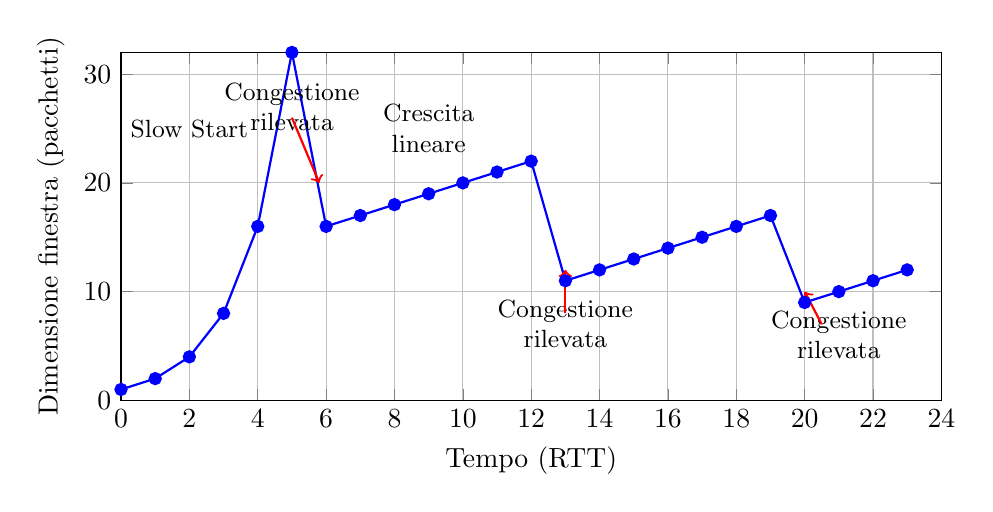
\begin{tikzpicture}
        \begin{axis}[
            width=12cm,
            height=6cm,
            grid=both,
            xlabel={Tempo (RTT)},
            ylabel={Dimensione finestra (pacchetti)},
            xmin=0, xmax=24,
            ymin=0, ymax=32,
            legend pos=north west
        ]
        
        % Fase di Slow Start e prima congestione
        \addplot[thick, blue, mark=*] coordinates {
            (0,1) (1,2) (2,4) (3,8) (4,16) (5,32) (6,16) (7,17) (8,18) (9,19) 
            (10,20) (11,21) (12,22) (13,11) (14,12) (15,13) (16,14) (17,15) 
            (18,16) (19,17) (20,9) (21,10) (22,11) (23,12)
        };
        
        % Annotazioni posizionate per evitare sovrapposizioni
        \node[align=center, text width=2cm, font=\small] at (axis cs:2,25) {Slow Start};
        
        \node[align=center, text width=2.5cm, font=\small] at (axis cs:9,25) {Crescita\\lineare};
        
        \node[align=center, text width=2.5cm, font=\small] at (axis cs:5,27) {Congestione\\rilevata};
        
        \node[align=center, text width=2.5cm, font=\small] at (axis cs:13,7) {Congestione\\rilevata};
        
        \node[align=center, text width=2.5cm, font=\small] at (axis cs:21,6) {Congestione\\rilevata};
        
        % Frecce che puntano ai punti di congestione
        \draw[->, thick, red] (axis cs:5,26) -- (axis cs:5.8,20);
        \draw[->, thick, red] (axis cs:13,8) -- (axis cs:13,12);
        \draw[->, thick, red] (axis cs:20.5,7) -- (axis cs:20,10);
        
        \end{axis}
    \end{tikzpicture}
    \caption{Evoluzione della dimensione della finestra di congestione nel tempo}
\end{figure}

\subsection{Esempio Concreto}
Immaginiamo un trasferimento di un file da un server a Milano a un client a New York:

\begin{enumerate}
    \item \textbf{Inizio prudente:} Il server inizia inviando solo 2 pacchetti (10KB).
    \item \textbf{Feedback positivo:} Ricevuti ACK senza problemi, raddoppia a 4 pacchetti (20KB).
    \item \textbf{Crescita esponenziale:} Continua a raddoppiare: 8, 16, 32 pacchetti.
    \item \textbf{Congestione:} A 32 pacchetti (160KB), alcuni router tra Milano e NY iniziano a scartare pacchetti perché sovraccarichi.
    \item \textbf{Rilevamento:} Il server rileva la perdita (timeout o ACK duplicati).
    \item \textbf{Adattamento:} Riduce la finestra a 16 pacchetti e passa a crescita lineare.
    \item \textbf{Crescita cauta:} Aumenta di 1 pacchetto per RTT: 17, 18, 19...
    \item \textbf{Stabilizzazione:} Trova il punto di equilibrio tra velocità massima e congestione della rete.
\end{enumerate}

Questo meccanismo adattivo è ciò che permette a TCP di trovare automaticamente la velocità ottimale di trasmissione in qualsiasi condizione di rete, adattandosi dinamicamente a cambiamenti di congestione, larghezza di banda o latenza.

\section{Nomi di Dominio e Servizio DNS (Domain Name System)}
\begin{itemize}
    \item \textbf{Problema:} Utenti usano nomi (es. \texttt{www.google.com}), rete usa IP.
    \item \textbf{Nomi di Dominio:} Gerarchici, es. \texttt{www.informatica.unibo.it}.
    \item \textbf{Servizio DNS:} Risolve nomi di dominio in indirizzi IP.
    \begin{itemize}
        \item \textbf{Gerarchia di Server DNS:} Radice, TLD, Autoritativi, Locali/Ricorsivi.
        \item \textbf{Processo di Risoluzione:} Il resolver locale interroga la gerarchia fino a ottenere l'IP.
    \end{itemize}
\end{itemize}

\section{Livello Applicazione}
\begin{itemize}
    \item \textbf{Scopo:} Fornire primitive e protocolli per le applicazioni di rete.
    \item \textbf{Relazione con Livelli Inferiori:} Si appoggia su Livello Trasporto (TCP/UDP).
    \item \textbf{Esempi di Protocolli e Applicazioni:}
    \begin{itemize}
        \item \textbf{Posta Elettronica (E-mail):} \texttt{SMTP} (invio, TCP 25), \texttt{POP3} (ricezione, TCP 110), \texttt{IMAP} (gestione su server, TCP 143).
        \item \textbf{World Wide Web (WWW):} \texttt{HTTP} (TCP 80), \texttt{HTTPS} (TCP 443).
        \item \textbf{DNS:} Protocollo DNS stesso (UDP 53 principalmente).
    \end{itemize}
\end{itemize}

\section{Servizi Client/Server e Peer-to-Peer (P2P)}
\begin{itemize}
    \item \textbf{Architettura Client/Server:}
    \begin{itemize}
        \item \textbf{Client:} Richiedono servizi. \textbf{Server:} Forniscono servizi.
        \item Esempi: DNS, Web, E-mail.
    \end{itemize}
    \item \textbf{Architettura Peer-to-Peer (P2P):}
    \begin{itemize}
        \item Tutti gli host (\textbf{peer}) sono sia client che server.
        \item Esempi: File-sharing (BitTorrent), alcune criptovalute.
    \end{itemize}
    \item \textbf{Servizi Ibridi:} Elementi di entrambe; server centrali per coordinamento, scambio dati P2P.
    \begin{itemize}
        \item Esempio: Napster (originale).
    \end{itemize}
\end{itemize}

\section{Configurazione TCP/IP (Host per Connessione a Internet)}
\begin{itemize}
    \item \textbf{Riassunto:} Cosa serve per configurare un host (es. PC domestico) per Internet via ISP.
    \item \textbf{Passi e Componenti:}
    \begin{enumerate}
        \item \textbf{Installare Dispositivo/Scheda di Rete} (Modem, Ethernet/Wi-Fi).
        \item \textbf{Stack Protocollare:} TCP/IP (e \texttt{PPP} per modem).
        \item \textbf{Firewall} (Raccomandato).
        \item \textbf{Informazioni di Configurazione} (manuale o via DHCP dall'ISP):
        \begin{itemize}
            \item Indirizzo IP dell'host.
            \item Maschera di Rete (Netmask).
            \item Indirizzo IP del Default Router (Gateway) dell'ISP.
            \item Indirizzo IP del/dei Server DNS dell'ISP.
            \item (Opzionale) IP server SMTP, POP3, IMAP.
        \end{itemize}
    \end{enumerate}
\end{itemize}

\section{Cenni sulla Sicurezza in Rete}
\begin{itemize}
    \item \textbf{1. Prevenzione Programmi Dannosi (Malware, Virus):}
    \begin{itemize}
        \item Difesa: Antivirus, buone pratiche.
    \end{itemize}
    \item \textbf{2. Controllo dell'Accesso a Sistemi di Rete Privati:}
    \begin{itemize}
        \item \textbf{Firewall:} Filtra pacchetti al perimetro della rete.
        \item \textbf{Autenticazione e Autorizzazione:} Per accessi consentiti (Login, Password, ACL).
        \item \textbf{Application Gateway (Proxy):} Server intermedio per controllo accessi a specifiche app.
    \end{itemize}
    \item \textbf{3. Segretezza (Privacy) dei Dati Trasmessi:}
    \begin{itemize}
        \item \textbf{Crittografia e Cifratura:} Trasformare dati in formato illeggibile senza chiave.
        \item Esempi: SSL/TLS (HTTPS), PGP, VPN.
    \end{itemize}
\end{itemize}

\section{Servizi Differenziati e Internet2}
\begin{itemize}
    \item \textbf{Criticità di Internet Tradizionale:} Mancanza di Garanzie sulla Qualità del Servizio (QoS).
    \begin{itemize}
        \item TCP affidabile, ma non garantisce \textit{quando} i pacchetti arrivano.
        \item Router tradizionali trattano tutti i pacchetti "best-effort".
    \end{itemize}
    \item \textbf{Internet2 e Servizi Differenziati (IntServ, DiffServ):}
    \begin{itemize}
        \item \textbf{Scopo:} Supportare app con requisiti QoS stringenti.
        \item \textbf{Approccio:} Nuova infrastruttura, router intelligenti, prioritizzazione, riservazione risorse, classificazione/marcatura pacchetti.
        \item \textbf{Obiettivo:} Garantire QoS su tutto il collegamento.
    \end{itemize}
\end{itemize}

\section{Recap dei Concetti Chiave}

\subsection{Principi Fondamentali e Architettura}
\begin{itemize}
    \item \textbf{Reti di Reti (Internetworking):} LAN interconnesse tramite \textbf{router} e \textbf{dorsali (backbone)}. I router operano al \textbf{Livello 3 (Rete)} e astraggono i dettagli delle LAN sottostanti.
    \item \textbf{Protocollo IP (Internet Protocol):}
    \begin{itemize}
        \item Fornisce \textbf{indirizzamento IP} globale e gerarchico.
        \item Gestisce l'\textbf{instradamento (forwarding)} dei pacchetti in modo \textbf{connectionless}.
        \item Include \textbf{frammentazione} e un \textbf{header IP} con indirizzi mittente/destinatario.
    \end{itemize}
    \item \textbf{Indirizzamento IPv4:}
    \begin{itemize}
        \item Formato: 32 bit (4 byte), es. \texttt{192.168.1.1}.
        \item Struttura: \textbf{Network Number} + \textbf{Host Number}.
        \item Classi (A, B, C): Schema storico basato sul primo byte (oggi si usa CIDR).
    \end{itemize}
    \item \textbf{Sottoreti (Subnetting):}
    \begin{itemize}
        \item \textbf{Subnet Mask:} Divide l'indirizzo IP in parte rete e parte host.
        \item Permette una gestione gerarchica e più efficiente degli indirizzi.
        \item Configurazione Host: \textbf{IP, Subnet Mask, Default Gateway}.
    \end{itemize}
\end{itemize}

\subsection{Instradamento e Controllo}
\begin{itemize}
    \item \textbf{Forwarding vs. Routing:}
    \begin{itemize}
        \item \textbf{Forwarding:} Decisione di inoltro basata sulla tabella di routing esistente.
        \item \textbf{Routing:} Processo di costruzione e aggiornamento delle tabelle di routing (es. RIP, OSPF, BGP).
    \end{itemize}
    \item \textbf{ICMP (Internet Control Message Protocol):} Per messaggi di controllo ed errore (non dati utente).
    \begin{itemize}
        \item Usato da \textbf{PING} (test connettività, RTT) e \textbf{Traceroute} (scoperta percorso).
    \end{itemize}
    \item \textbf{ARP (Address Resolution Protocol):} Risolve indirizzi IP in indirizzi MAC su una LAN.
    \begin{itemize}
        \item Funziona con ARP Request (broadcast) e ARP Reply (unicast).
        \item Mantiene una \textbf{ARP Cache}.
        \item \textbf{RARP} (Reverse ARP): Obsoleto, per ottenere IP da MAC.
    \end{itemize}
    \item \textbf{DHCP (Dynamic Host Configuration Protocol):} Assegna automaticamente IP e altre configurazioni (netmask, gateway, DNS) ai client. Processo DORA (Discover, Offer, Request, Acknowledge).
\end{itemize}

\subsection{Transizione e Livello Trasporto}
\begin{itemize}
    \item \textbf{IPv6:} Indirizzi a 128 bit per superare esaurimento IPv4. Coesistenza con IPv4 tramite \textbf{tunnelling}.
    \item \textbf{Livello Trasporto:} Comunicazione end-to-end tra applicazioni.
\end{itemize}
\begin{table}[H]
    \centering
    \begin{tabular}{|l|p{5cm}|p{5cm}|}
        \hline
        \rowcolor{bg_custom}
        \textbf{Caratteristica} & \textbf{TCP (Transmission Control Protocol)} & \textbf{UDP (User Datagram Protocol)} \\
        \hline
        Affidabilità & Alta (garantisce consegna ordinata, ritrasmissione) & Bassa (best-effort, no garanzie) \\
        \hline
        Connessione & Orientato alla connessione (handshake) & Connectionless \\
        \hline
        Overhead & Più alto & Più basso \\
        \hline
        Controllo Flusso & Sì (Sliding Window) & No \\
        \hline
        Controllo Congestione & Sì (Sliding Window variabile) & No \\
        \hline
        Uso Tipico & Web (HTTP/S), Email (SMTP), FTP & Streaming, DNS, Giochi online, VoIP \\
        \hline
    \end{tabular}
    \caption{Confronto TCP vs UDP}
\end{table}
\begin{itemize}
    \item \textbf{Socket:} Punto di comunicazione (coppia \texttt{Indirizzo IP : Numero di Porta}).
    \item \textbf{Controllo Flusso/Congestione (TCP):}
    \begin{itemize}
        \item \textbf{Finestra Scorrevole (Sliding Window):} Quantità di dati inviabili prima di un ACK.
        \item Adattamento dinamico della finestra per evitare di sovraccaricare destinatario (flusso) o rete (congestione). Fasi: Slow Start, Crescita Additiva, Riduzione Moltiplicativa.
    \end{itemize}
\end{itemize}

\subsection{Servizi e Protocolli Applicativi}
\begin{itemize}
    \item \textbf{DNS (Domain Name System):} Risolve nomi di dominio (es. \texttt{www.unibo.it}) in indirizzi IP. Struttura gerarchica di server.
    \item \textbf{Livello Applicazione:} Protocolli specifici per diverse applicazioni:
    \begin{itemize}
        \item \textbf{Email:} SMTP (invio), POP3/IMAP (ricezione).
        \item \textbf{Web:} HTTP/HTTPS.
    \end{itemize}
    \item \textbf{Architetture Applicative:}
    \begin{itemize}
        \item \textbf{Client/Server:} Client richiedono, Server forniscono (es. Web).
        \item \textbf{Peer-to-Peer (P2P):} Ogni nodo è sia client che server (es. BitTorrent).
    \end{itemize}
\end{itemize}

\subsection{Configurazione, Sicurezza e QoS}
\begin{itemize}
    \item \textbf{Configurazione TCP/IP Host:}
    \begin{enumerate}
        \item Indirizzo IP
        \item Subnet Mask
        \item Default Gateway
        \item Server DNS
    \end{enumerate}
    \item \textbf{Sicurezza in Rete:}
    \begin{itemize}
        \item Prevenzione \textbf{malware}.
        \item Controllo accessi: \textbf{Firewall} (filtra pacchetti), Autenticazione/Autorizzazione.
        \item Privacy: \textbf{Crittografia} (es. HTTPS).
    \end{itemize}
    \item \textbf{Qualità del Servizio (QoS) e Internet2:}
    \begin{itemize}
        \item Internet tradizionale: "best-effort", senza garanzie sui tempi.
        \item Internet2 e Servizi Differenziati mirano a fornire QoS tramite router intelligenti, priorità e riservazione risorse.
    \end{itemize}
\end{itemize}

\end{document}